\documentclass[../main.tex]{subfiles}

\begin{document}

% -----------------------
% Definición del concepto
% -----------------------
\subsubsection{Definición del concepto.}
La denominada como \acrfull{eIDAS} es el intento de la Unión Europea de establecer el paradigma de la \acrfull{SSI} a todos sus ciudadanos, residentes y empresas, para que de tal manera ``puedan beneficiarse de una cartera de identidad digital europea personal a partir de 2026''  \cite{DigitalIdentityRegulation}.
\\

Entre los servicios y herramientas que se pretenden poder utilizar destacan los siguientes: ``Firma electrónica, Sello de tiempo, Identificación electrónica, Certificado cualificado de autenticación de sitio web, Sello electrónico y Servicio de entrega electrónica certificada'' \cite{EuropeanDigitalIdentity}.
\\

Para ello, el denominado como \textbf{eIDAS Bridge} asistirá a los Emisores ayudando durante el firmado y a los Verificadores mediante la automatización del proceso de identificación de la organización tras el \acrshort{DID} del Emisor \cite{SSIeIDAS}. Podemos entenderlo como una manera de comprobar si una determinada \acrshort{VC} tiene validez (sea de confianza) para ser empleada en la Unión Europea. 
\\

\begin{figure}[htbp]
    \centering
    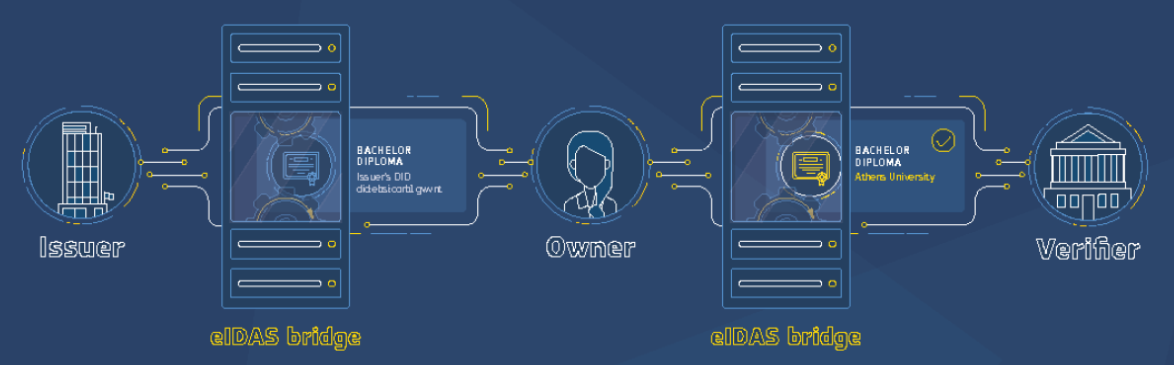
\includegraphics[width=1\linewidth]{images/eIDAS.png}
    \caption{\textit{Modo de funcionamiento del eIDAS Bridge.} Fuente \cite{SSIeIDAS}}
    \label{fig:eIDAS}
\end{figure}


% -----------------------------------------------
% Infraestructura Europea de Servicios Blockchain
% -----------------------------------------------
\newpage
\subsubsection{Infraestructura Europea de Servicios Blockchain.}
El anteriormente mencionado \textbf{eIDAS Bridge} forma parte del \acrfull{ESSIF} y es uno de los principales casos de uso de la \acrfull{EBSI} \cite{SSIeIDAS}, la cual es una iniciativa de la Comisión Europea y de la Asociación Europea de Blockchain para la implantación del paradigma al gran público.
\\

Analizando lo propuesto, vemos como se mantienen aspectos fundamentales  descritos con anterioridad. Sin embargo, es ahora la \acrshort{EBSI} quién se encarga de cumplimentar el rol de \acrshort{VDR}, tal y como se describe en su \textbf{Marco de Credenciales Verificables} \cite{ebsiVCF}. Por lo tanto, la principal función de la organización es la de registrar en una base de datos, basada en Blockchain pública y por lo tanto descentralizada, las transacciones realizadas en el proceso de expedición y verificación de credenciales verificables.  
\\

\begin{figure}[htbp]
    \centering
    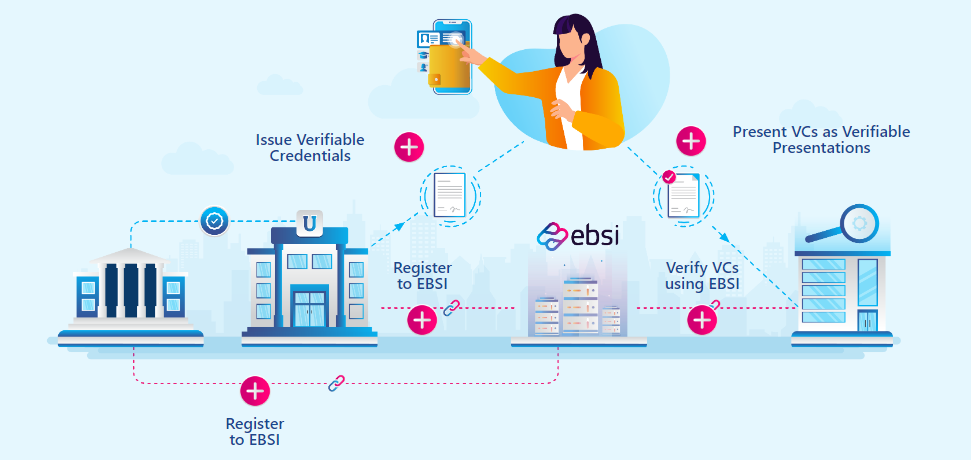
\includegraphics[width=1\linewidth]{images/EBSI.png}
    \caption{\textit{Papel de la \acrshort{EBSI} en el paradigma.} Fuente \cite{ebsiVCF}}
    \label{fig:EBSI}
\end{figure}

\refstepcounter{observacion}
\begin{tcolorbox}[colback=gray!10!white, colframe=gray!50!black, title=Observación \theobservacion]\label{observacion-europa}
Destacar la distinción que se realiza en \cite{w3c} entre `persona natural' y `entidad legal', donde podemos encontrar información detallada de la adecuación del paradigma al ámbito legal europeo a causa del \acrfull{GDPR}.
\end{tcolorbox} 


% ------------------------------------
% Cartera de Identidad Digital Europea
% ------------------------------------
\newpage
\subsubsection{Cartera de Identidad Digital Europea.}

Actualmente, uno de los principales esfuerzos que se está llevando a cabo es el desarrollo de la \acrfull{EUDI Wallet}, la cual ya se está probando en entornos reales mediante cuatro proyectos a gran escala que se lanzaron el 1 de abril de 2023 \cite{EuropeanDigitalIdentity}. 
\\

La principal fuente de información sobre los detalles de su implementación es \cite{EUDigitalIdentityWalletArchitecture}, donde se puede encontrar el repositorio informativo raíz de la iniciativa en \Gls{Github}. Allí se describen aspectos fundamentales de la misma como una descripción del ecosistema, el establecimiento de los principales casos de uso o la definición de la \textbf{Arquitectura y Marco de Referencia} junto con sus componentes. En los numerosos repositorios pertenecientes a la organización se alojan las diferentes librerías elaboradas para la creación de una \textbf{aplicación móvil} para Android y IOS que permite a los usuarios gestionar sus credenciales.
\\

\begin{figure}[htbp]
    \centering
    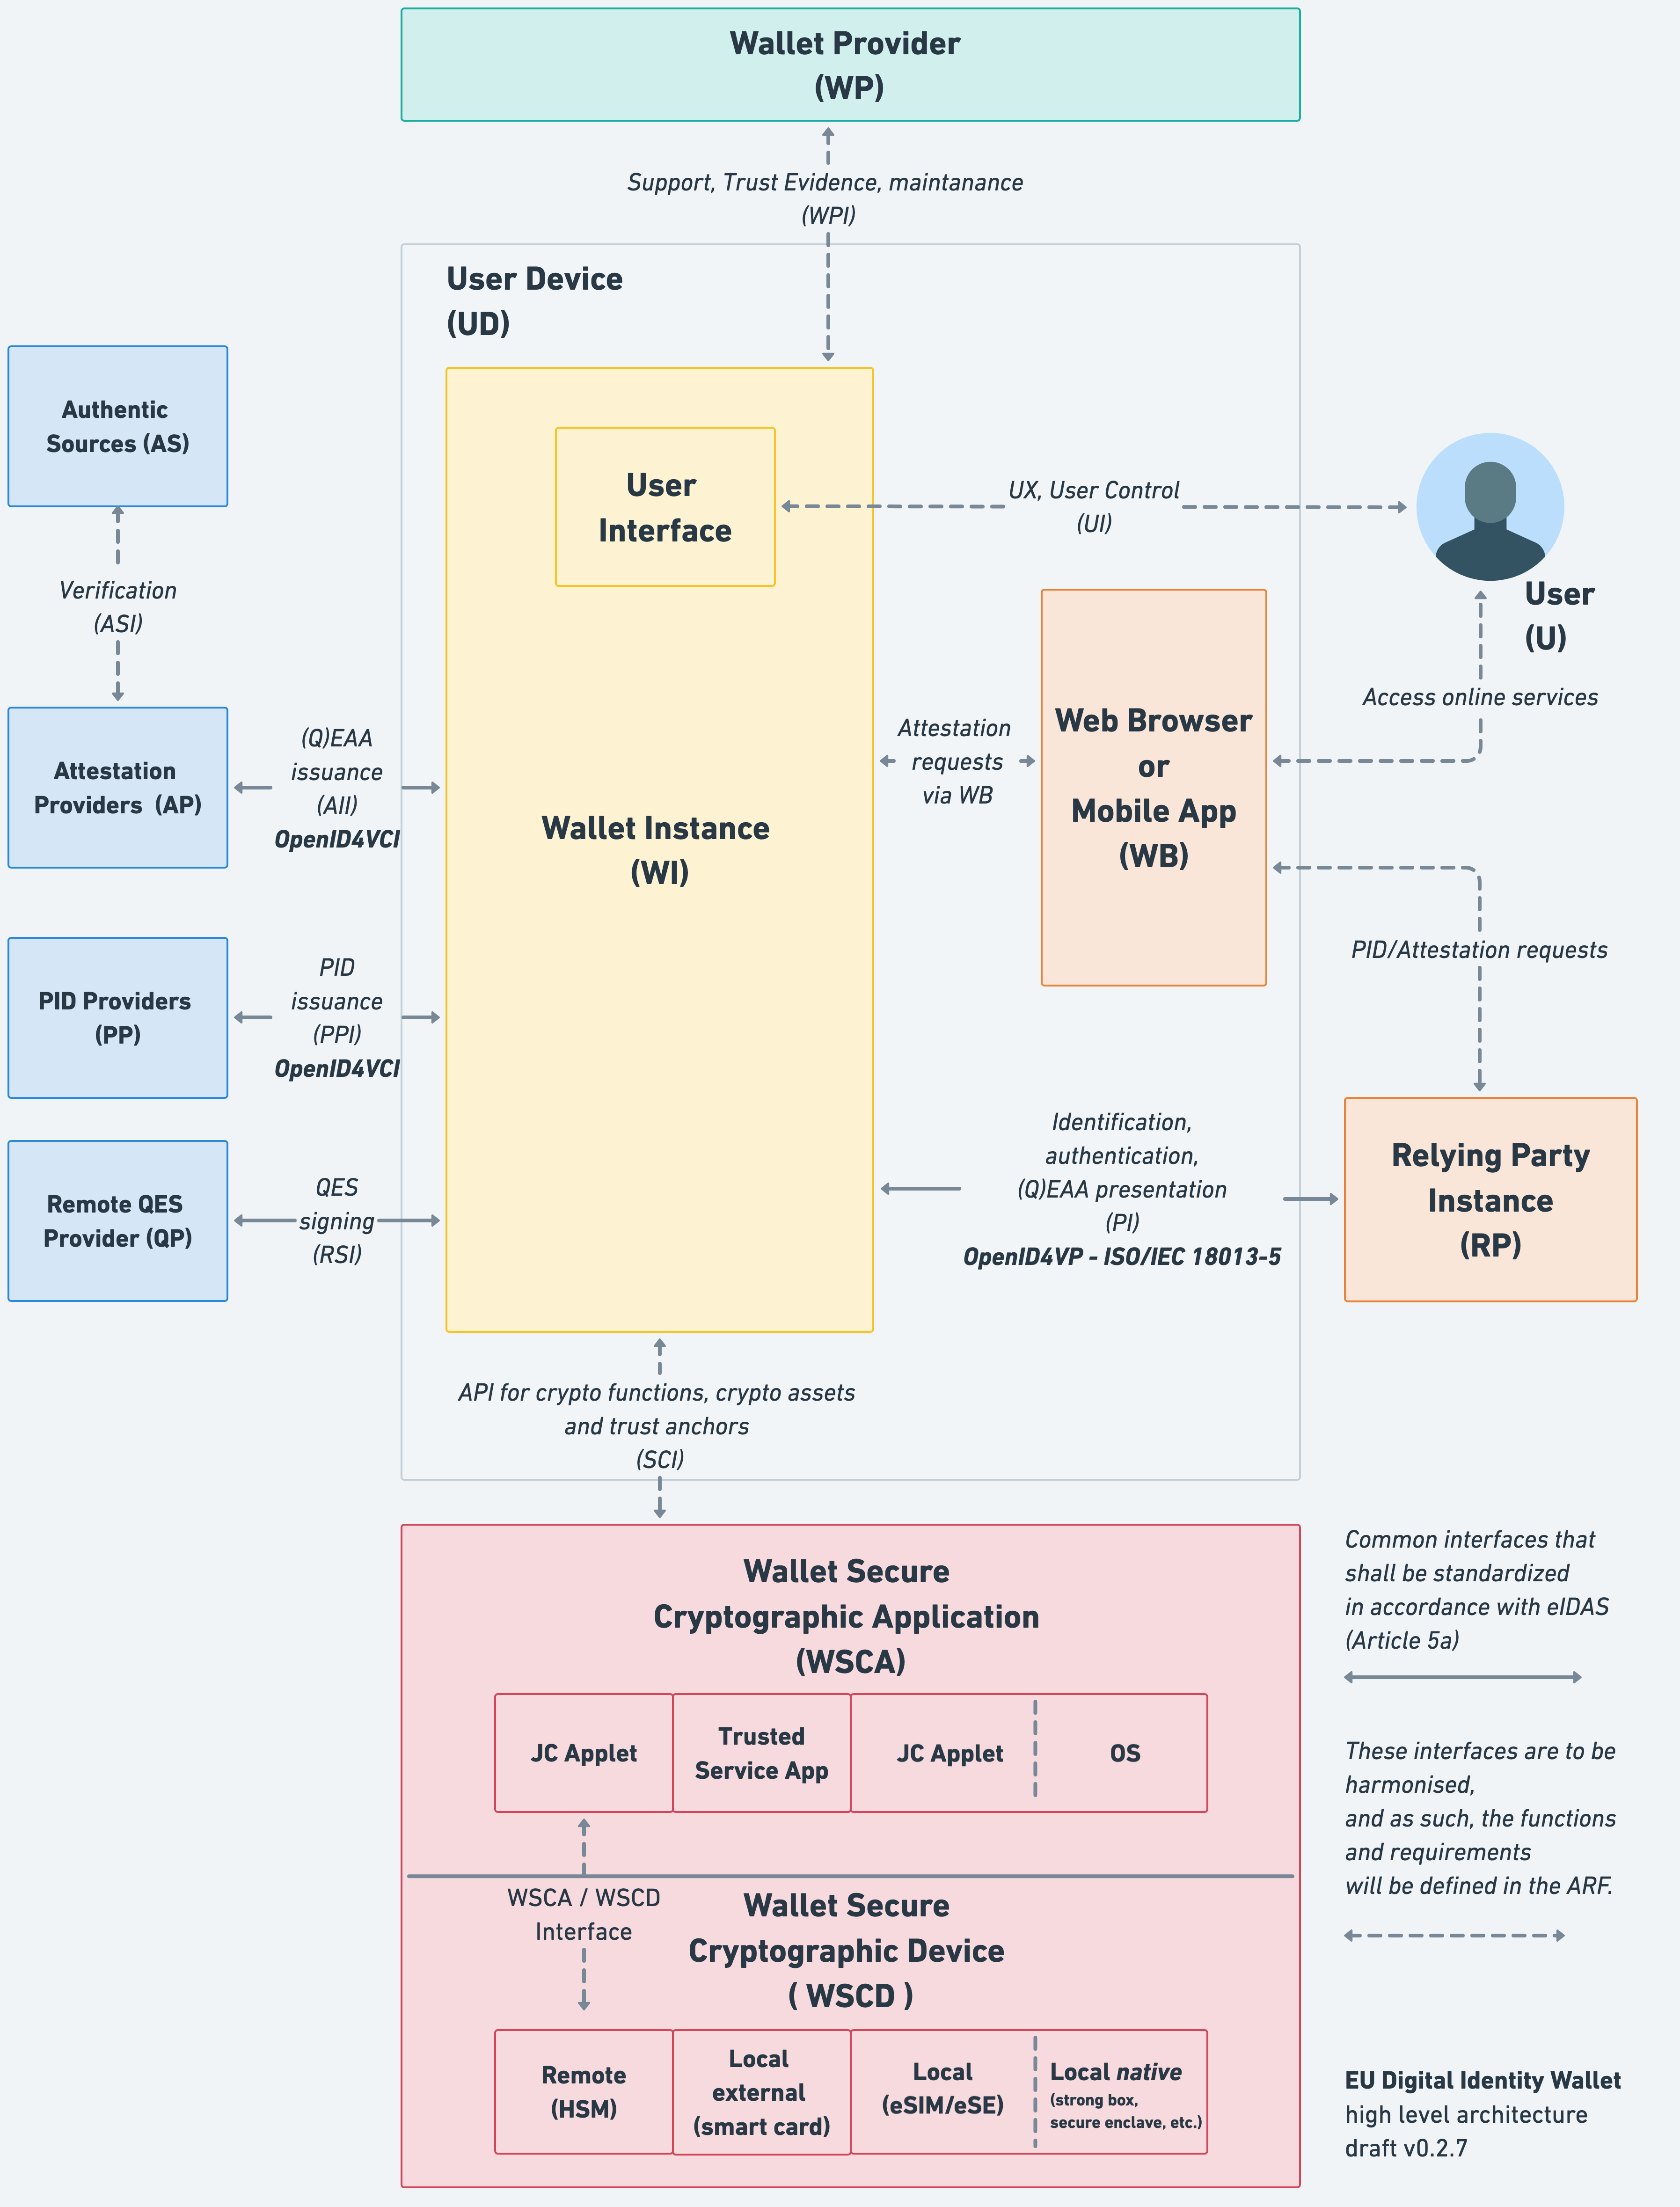
\includegraphics[width=0.55\linewidth]{images/EUDI_Ecosystem.png}
    \caption{\textit{Arquitectura de la \acrshort{EUDI Wallet}.} Fuente \cite{EUDigitalIdentityWalletArchitecture}}
    \label{fig:EUDI_Ecosystem}
\end{figure}


\end{document}